\subsection*{Broken Access Control -- Privilege Escalation via Registration (BAC)}

\begin{table}[H]
\centering
\begin{tabular}{|l|p{10cm}|}
\hline
\textbf{Finding ID} & BAC \\
\hline
\textbf{Severity} & Critical \\
\hline
\textbf{CVSS 3.1 Score} & 9.8 (Critical) \\
\hline
\textbf{CVSS Vector} & \texttt{AV:N/AC:L/PR:N/UI:N/S:U/C:H/I:H/A:H} \\
\hline
\textbf{Status} & Confirmed \\
\hline
\textbf{OWASP Category} & A01:2021 -- Broken Access Control \\
\hline
\textbf{CWE} & CWE-269 -- Improper Privilege Management \\
\hline
\textbf{Affected Endpoint} & \texttt{POST /api/Users/} \\
\hline
\textbf{Affected Parameter} & \texttt{role} \\
\hline
\end{tabular}
\caption{Broken Access Control -- Privilege Escalation finding details}
\end{table}

\subsubsection*{Description}

The user registration function was found to accept a \texttt{role}
field directly from the client without server-side restriction.

By intercepting the registration request and modifying this field, a
normal user was able to register a new account with administrator
privileges. The server did not validate whether the client was
authorized to set this value, allowing any unauthenticated visitor to
create an admin-level account.

\subsubsection*{Methodology}

The registration functionality was tested by creating a normal user
account while intercepting the registration request using Burp Suite.
The request body was reviewed to identify client-controlled parameters
that could affect account privileges. The \texttt{role} parameter was
then modified from its normal value to \texttt{admin} and the modified
request was forwarded to the server.

The resulting account was subsequently used to verify whether
administrator-level access had been granted. Successful access to the
Administration page confirmed that the server accepted the
client-supplied role without performing adequate server-side
authorization checks.

\subsubsection*{Steps to Reproduce}

\begin{enumerate}
    \item Navigate to the registration page and begin creating a new
    account normally.

    \item Intercept the registration request using Burp Suite before
    it reaches the server.

    \item Modify the request body to include the following field:

    \begin{lstlisting}
"role": "admin"
    \end{lstlisting}

    \item Forward the modified request to the server.

    \item Log in using the newly created account
    (\texttt{User14@gmail.com}).

    \item Verify that the account can access the Administration page
    and its associated functionality.
\end{enumerate}

\subsubsection*{Evidence}

\begin{figure}[H]
    \centering
    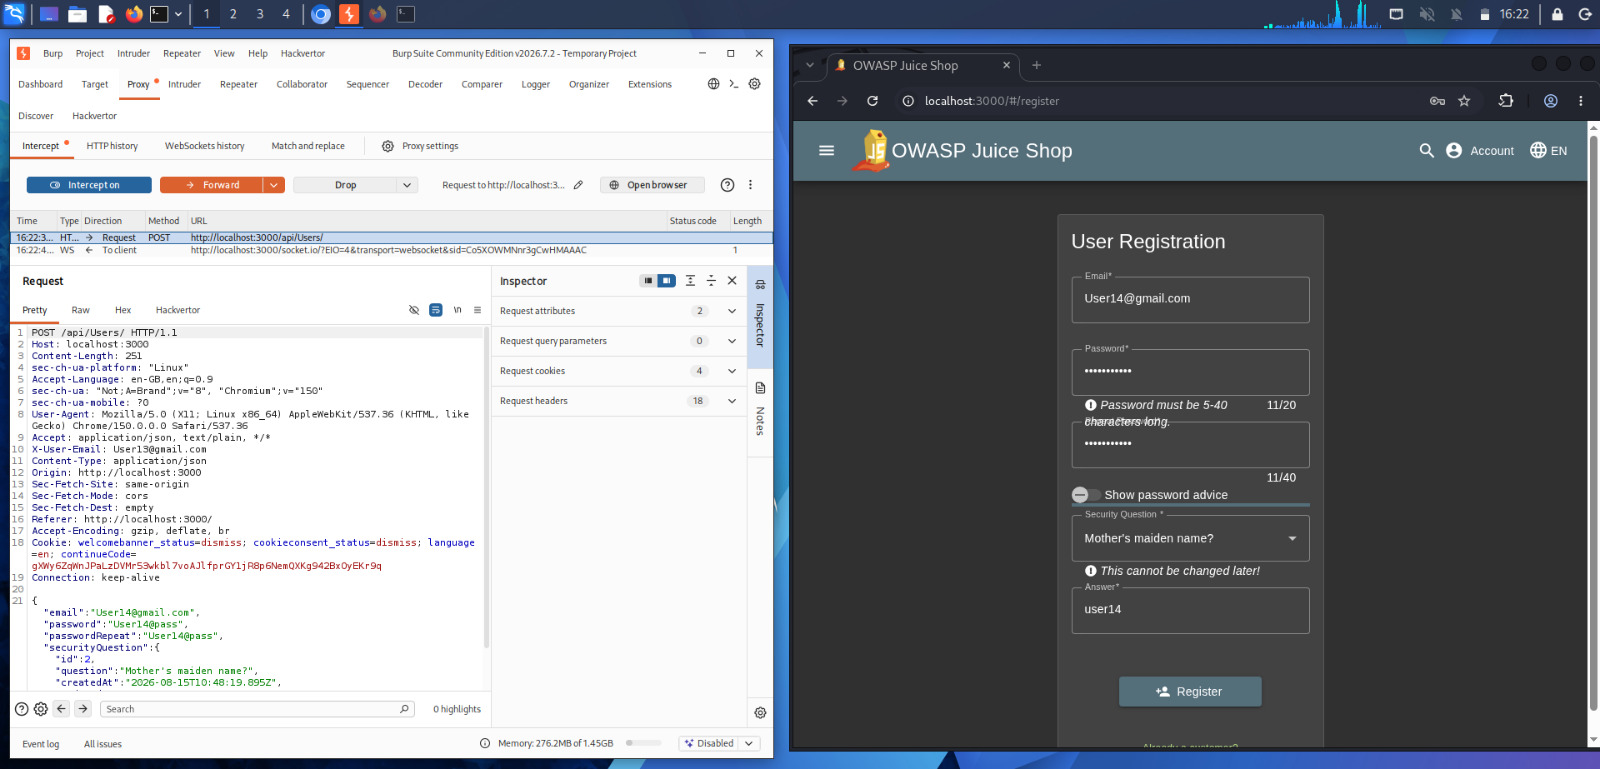
\includegraphics[width=0.8\textwidth]
    {evidence/phase4/bac/bac01-burp-registration-request.jpg}
    \caption{Registration request captured in Burp Suite}
\end{figure}

\begin{figure}[H]
    \centering
    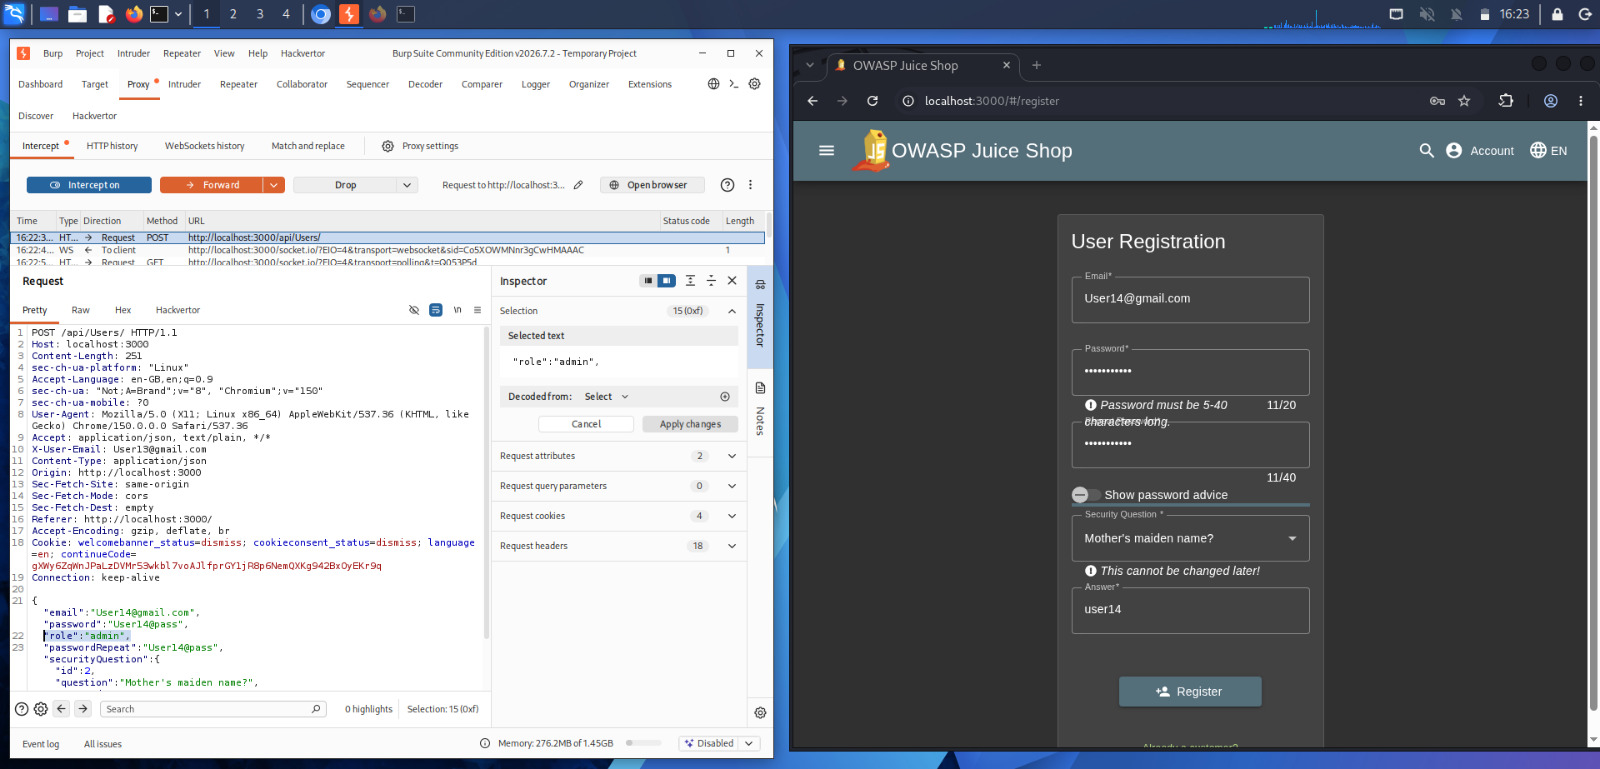
\includegraphics[width=0.8\textwidth]
    {evidence/phase4/bac/bac02-burp-role-admin-modification.jpg}
    \caption{Registration request modified to set the role to admin}
\end{figure}

\begin{figure}[H]
    \centering
    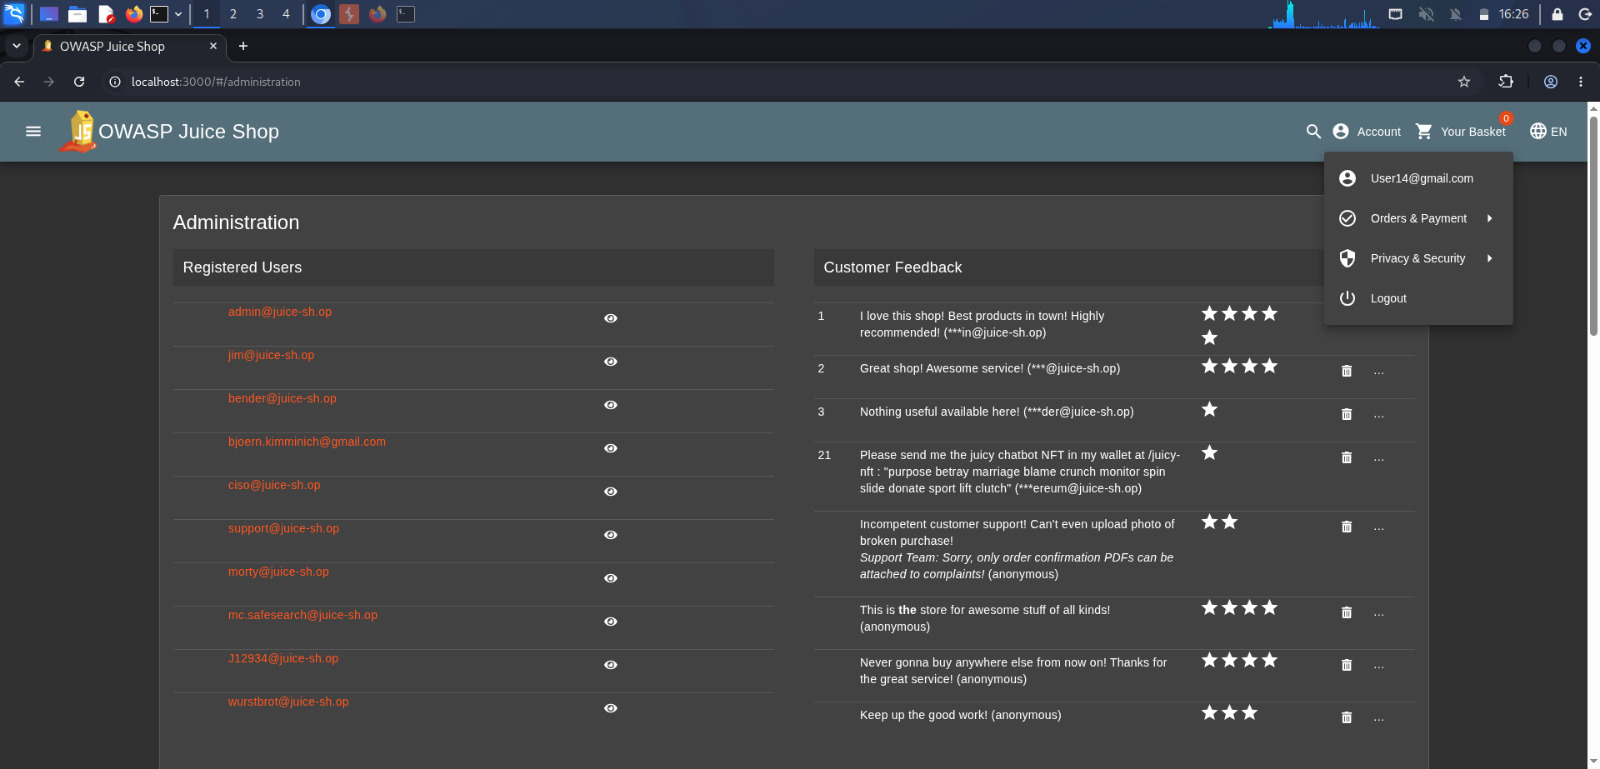
\includegraphics[width=0.8\textwidth]
    {evidence/phase4/bac/bac03-admin-page-access.jpg}
    \caption{Newly created account successfully accessing the Administration page}
\end{figure}

\begin{figure}[H]
    \centering
    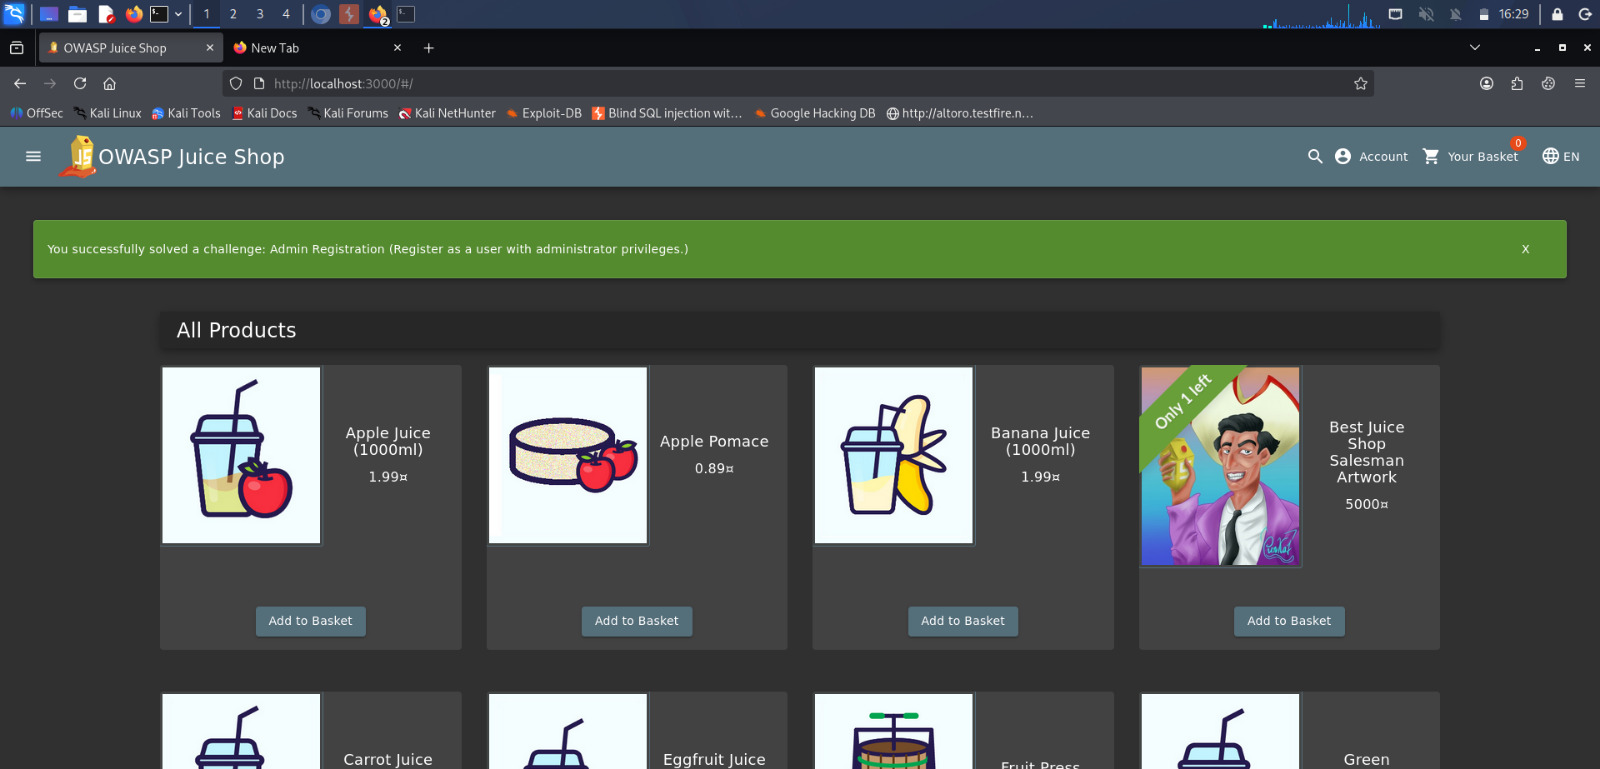
\includegraphics[width=0.8\textwidth]
    {evidence/phase4/bac/bac04-admin-registration-challenge-success.jpg}
    \caption{Successful completion of the Admin Registration challenge}
\end{figure}

\subsubsection*{Impact}

An attacker can create an administrator account without authorization.
After logging in with the new account, the attacker can access
administrator functions that should only be available to authorized
administrators.

This can allow unauthorized management of users, products, and other
administrative data.

\subsubsection*{Remediation}

\begin{itemize}
    \item Do not allow users to choose their role during registration.
    \item Always assign the normal user role on the server side when
    creating a new account.
    \item Ignore or reject any client-supplied \texttt{role} value
    during normal registration.
    \item Allow only authorized administrators to change a user's role.
    \item Perform server-side authorization checks before allowing
    access to administrator functions.
\end{itemize}

\subsubsection*{Conclusion}

The Broken Access Control vulnerability was successfully confirmed by
modifying the registration request and assigning the \texttt{admin}
role to a newly created account.

The account was then able to access the Administration page,
confirming that the application does not properly enforce server-side
privilege controls during registration.

The finding is therefore classified as a confirmed Critical-severity
security issue.